\section{Introduction}
\subsection{Background}
\frame
{
\frametitle{Background}
\begin{block}{}
A fundamental engineering challenge surrounding brittle materials is predicting failure. This involves predicting where fractures \textbf{nucleate} as well as how these fractures \textbf{propagate}.
\newline
\newline
Researchers at Sandia National Laboratories have used Molecular Dynamics (MD) simulations to model the effects that cause nucleation and growth, but this is computationally intensive.
\end{block}
}

%%%%%%%%%%%%%%%%%%%%%%%%%%%%%%%%%%%%%%%%%%%%%%%%%%%%%%%%%%%%%%%%%%%%%%%%%%%%%%%%%%%%%%%%%

\frame{
\frametitle{ Sandia National Laboratories}
\begin{minipage}[0.2\textheight]{\textwidth}
\begin{columns}[T]
    \begin{column}{0.5\textwidth}
    
  \begin{block}{}
    \textbf{Sandia's Interest:} Brittle materials are used throughout the stockpile. Examples include headers, electronic connectors, etc. 
    \newline
    \newline
    \textbf{Challenge:} Make reliability predictions for components containing brittle materials. 
  \end{block}
    \end{column}
    
    \begin{column}{0.5\textwidth}
    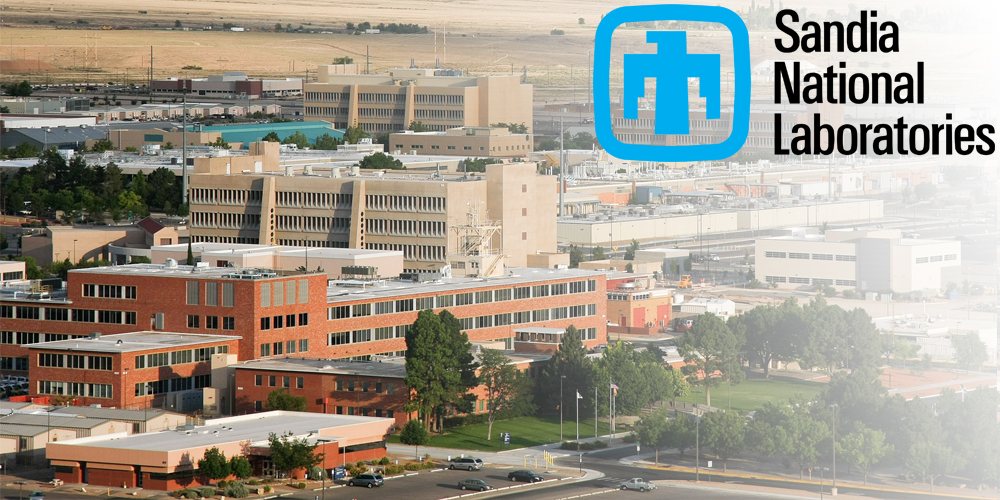
\includegraphics[width=5.5cm]{images/sandia.jpg}
    \end{column}
\end{columns}
\end{minipage}
}

%%%%%%%%%%%%%%%%%%%%%%%%%%%%%%%%%%%%%%%%%%%%%%%%%%%%%%%%%%%%%%%%%%%%%%%%%%%%%%%%%%%%%%%%%

\frame
{
\frametitle{Motivation}
\begin{block}{}
The clinic aims to develop a model that rapidly predicts where fractures will form silica-based glasses. We consider different environmental conditions including different boundary properties exposure to water.
\newline
\newline
By creating a graph theoretic description of the material we will train a supervised \textbf{Machine Learning (ML)} algorithm on MD simulation data.
\end{block}
}

%%%%%%%%%%%%%%%%%%%%%%%%%%%%%%%%%%%%%%%%%%%%%%%%%%%%%%%%%%%%%%%%%%%%%%%%%%%%%%%%%%%%%%%%%

\frame
{
\frametitle{Physical Structure}
   \begin{columns}
    	\begin{column}{.5\textwidth}
			\begin{figure}[!b]
    \centering
    \noindent
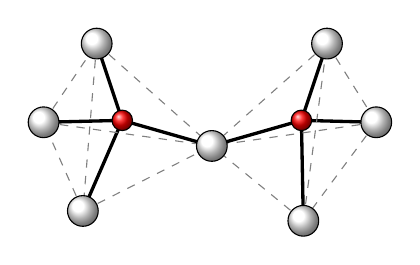
\begin{tikzpicture}[scale=.65]
\coordinate (A) at (-0.5,0.5,0); % Left back O 
\coordinate (B) at (2,0.5,4.5); % Left front O  
\coordinate (C) at (6,0.5,0); % Right back O
\coordinate (D) at (6.5,0.5,5); % Right front O 
\coordinate (E) at (3.75,1,2.5); % Bridging Oxygen 
\coordinate (F) at (5.5,1.5,2.5); % Right Si
\coordinate (G) at (2,1.5,2.5); % Left Si 
\coordinate (H) at (1.5,3,2.5); % Left top O 
\coordinate (I) at (6,3,2.5); % Right Top O

%connections from left Si
\draw [very thick] (G) -- (A);
\draw [very thick] (G) -- (B);
\draw [very thick] (G) -- (H);
\draw [very thick] (G) -- (E);

%connections from Right Si 
\draw [very thick] (F) -- (C);
\draw [very thick] (F) -- (D);
\draw [very thick] (F) -- (I);
\draw [very thick] (F) -- (E);

%dashed lines between Oxygen. This can be removed but it was in literature. 
\draw[gray,dashed] (A) -- (H);
\draw[gray,dashed] (H) -- (B);
\draw[gray,dashed] (B) -- (A);
\draw[gray,dashed] (A) -- (E);
\draw[gray,dashed] (H) -- (E);
\draw[gray,dashed] (B) -- (E);

\draw[gray,dashed] (I) -- (C);
\draw[gray,dashed] (C) -- (D);
\draw[gray,dashed] (D) -- (I);
\draw[gray,dashed] (I) -- (E);
\draw[gray,dashed] (D) -- (E);                                                
\draw[gray,dashed] (C) -- (E);  

%place non-atom cube corners
\shadedraw [ball color= white] (A) circle (0.3cm);
\shadedraw [ball color= white] (B) circle (0.3cm);
\shadedraw [ball color= white] (C) circle (0.3cm);
\shadedraw [ball color= white] (D) circle (0.3cm);
\shadedraw [ball color= white] (E) circle (0.3cm);
\shadedraw [ball color= red] (F) circle (0.20cm);
\shadedraw [ball color= red] (G) circle (0.20cm);
\shadedraw [ball color= white] (H) circle (0.3cm);
\shadedraw [ball color= white] (I) circle (0.3cm);
\end{tikzpicture}
    %\caption{Two silicon atoms (red)\\with surrounding oxygen atoms (grey) in tetrahedral configuration. A bridging %oxygen is at the center.}
    
    \label{fig:tetrahedra}
\end{figure}

    {\bf SiO$_\mathbf{2}$}: Two silicon atoms (red)\\with surrounding oxygen atoms (grey) in tetrahedral configuration. A bridging oxygen is at the center.
    
		\end{column}
   		\begin{column}{.6\textwidth}
        \begin{block}{}
		\begin{itemize} 
        \item Nucleation is related to atomic-scale defects or chemical bond weakness in the glass
		\begin{itemize} 
        \item The relationship between atomic structure and fracture behavior is complex 
		\end{itemize}
        \item Nucleation and propagation depend more on subtle characteristics of the local structure surrounding an atom\\
    \end{itemize}
    \end{block}
		\end{column}
	\end{columns}
}

%%%%%%%%%%%%%%%%%%%%%%%%%%%%%%%%%%%%%%%%%%%%%%%%%%%%%%%%%%%%%%%%%%%%%%%%%%%%%%%%%%%%%%%%%

\subsection{Previous Work}
\frame
{\frametitle{Molecular Dynamics Simulations}
\begin{block}{}
Molecular dynamics (MD) methods simulate the system at the nanoscale and model the individual chemical and physical interactions taking place in the material.
\newline
\newline
These simulations have successfully predicted a wide range of detailed
properties that cannot be obtained with continuum methods, and that are
consistent with experimental observations.
\end{block}
}

%%%%%%%%%%%%%%%%%%%%%%%%%%%%%%%%%%%%%%%%%%%%%%%%%%%%%%%%%%%%%%%%%%%%%%%%%%%%%%%%%%%%%%%%%

\frame
{
\frametitle{LAMMPS}
\begin{block}{} 

Sandia has developed molecular dynamics simulation software Large-scale Atomic/Molecular Massively Parallel Simulator.

Simulations are generated using the LAMMPS code. Each LAMMPS run simulates a sample of SiO2 containing approximately 70,000 atoms.
\end{block}
}

%%%%%%%%%%%%%%%%%%%%%%%%%%%%%%%%%%%%%%%%%%%%%%%%%%%%%%%%%%%%%%%%%%%%%%%%%%%%%%%%%%%%%%%%%





\subsection{Math Clinic Goals}
\frame
{\frametitle{Objective}
\begin{block}{}
\begin{itemize}
    \item Develop supervised learning methods, trained on MD simulation data, that generate rapid predictions of where and when atomic-scale fractures occur in samples of silicate glasses under stress. 

\item Generate predictions under multiple environmental conditions, validate on existing MD simulation results. 

\item Relate predictions to specific features characterizing local atomic structure.

\item Provide new insight into how local structure leads to fracture and failure.
\end{itemize}
\end{block}
}

\frame
{\frametitle{Goals}
\begin{block}{}

\textbf{Goal 1:} Predict fracture nucleation events.
\newline
\newline

\textbf{Goal 2:} Predict fracture propagation.

\end{block}
}